\documentclass[article]{jss}

\usepackage{amsmath,amssymb}
\usepackage{amsthm}
\usepackage{booktabs}
\usepackage{tikz}
\usetikzlibrary{shapes,positioning,fit,calc}

\newtheorem{proposition}{Proposition}

%% almost as usual
\author{Mohamad Yamen Al Mohamad\\University of Tabriz \AND
        Ali Akbar Heydari\\University of Tabriz \AND
        Hossein Jabbari Khamnei\\University of Tabriz}
\Plainauthor{Mohamad Yamen Al Mohamad, Ali Akbar Heydari, Hossein Jabbari Khamnei}

\title{\pkg{unitTransformDist}: A Distribution-Agnostic \proglang{R} Package for Unit-Interval Models via the Odds-Inverting Transform}
\Plaintitle{unitTransformDist: A Distribution-Agnostic R Package for Unit-Interval Models via the Odds-Inverting Transform}
\Shorttitle{unitTransformDist: Unit-Interval Models via the Odds-Inverting Transform}

\Abstract{
Data restricted to the open interval $(0,1)$ -- proportions, rates, and probabilities -- are commonly modelled in \proglang{R} with \pkg{betareg} (beta regression), \pkg{simplexreg} (simplex regression), or the recently released \pkg{gkwdist} (generalized Kumaraswamy family). Each of these packages targets one specific parametric family, fixed in advance by its authors. This paper introduces \pkg{unitTransformDist}, which instead constructs a $(0,1)$-valued distribution from an arbitrary base distribution on $(0,\infty)$ via the transform $Y = 1/(1+X)$, taking the base distribution's density, cumulative distribution function, quantile function, and random-generation function directly as arguments rather than selecting from a fixed registry. This design lets users plug in \proglang{R}'s built-in distributions or their own custom research distributions -- including ones with no closed-form quantile function -- without modifying any package code. We derive the transform's density, distribution, quantile, moment, and hazard relationships in general form, establish an invariance property of the likelihood under the transform that underlies every inferential routine in the package, and use it to document and empirically correct a subtle but consequential implementation error common to profile-likelihood confidence intervals: freezing nuisance parameters at their unconstrained maximum-likelihood estimate while profiling a parameter of interest, rather than re-optimizing them at each candidate value. A reproducible Monte Carlo study included in the package shows this mistake holds actual 95\% coverage near 54--61\% across sample sizes $n \in \{30,60,100,200\}$ for a two-parameter gamma base distribution, essentially independent of $n$, while the corrected procedure restores coverage to 90--94\%; a further study across three base families shows the size of this effect depends on the correlation structure of the likelihood and is not universal. The package also provides Monte Carlo utilities for studying estimator bias and several bias-correction methods (jackknife, bootstrap, Firth-type), an experimental analytic bias-correction routine that we explicitly flag as unverified, and a small suite of diagnostics. We describe the package's design, its relationship to a broader literature of unit-interval distributions and \proglang{R} packages, its performance characteristics, and its current limitations, reporting negative and inconclusive results alongside positive ones.
}

\Keywords{unit interval, bounded distributions, odds transform, profile likelihood, Monte Carlo, bias correction, \proglang{R}}
\Plainkeywords{unit interval, bounded distributions, odds transform, profile likelihood, Monte Carlo, bias correction, R}

%% publication information, left for the technical editor
%% \Volume{}
%% \Issue{}
%% \Month{}
%% \Year{}
%% \Submitdate{}
%% \Acceptdate{}

\Address{
  Mohamad Yamen Al Mohamad\\
  Department of Statistics\\
  Faculty of Mathematics, Statistics, and Computer Sciences\\
  University of Tabriz\\
  Tabriz, Iran\\
  E-mail: \email{yamenmohamad@tabrizu.ac.ir}\\

  Ali Akbar Heydari\\
  Department of Statistics\\
  Faculty of Mathematics, Statistics, and Computer Sciences\\
  University of Tabriz\\
  Tabriz, Iran\\
  E-mail: \email{heydari@tabrizu.ac.ir}\\

  Hossein Jabbari Khamnei\\
  Department of Statistics\\
  Faculty of Mathematics, Statistics, and Computer Sciences\\
  University of Tabriz\\
  Tabriz, Iran\\
  E-mail: \email{h\_jabbari@tabrizu.ac.ir}
}

\begin{document}

\section{Introduction}
\label{sec:intro}

Continuous data confined to the open unit interval $(0,1)$ arise throughout applied statistics: disease prevalence, vote shares, market shares, budget allocations, normalized indices such as the Gini coefficient, and proportions of any kind are all naturally modelled as values strictly between zero and one. The Beta distribution has long served as the canonical model for such data \citep{johnsonkotzbalakrishnan1994}, and \proglang{R} has a mature ecosystem built around it and its relatives. \pkg{betareg} implements beta regression, linking the mean and precision of a Beta-distributed response to covariates through a generalized-linear-model-style linear predictor \citep{ferrari2004beta,cribarineto2010betareg}, later extended to mixtures, extended-support variants, and partitioned models \citep{gruen2012betareg}, and closely related proposals appear under different names in \citet{kieschnick2003} and \citet{smithsonverkuilen2006}. \pkg{simplexreg} instead models the response as simplex-distributed, following \citet{songtan2000} and implemented for \proglang{R} by \citet{zhang2016simplexreg}, with maximum likelihood and generalized estimating equations for longitudinal data. The Kumaraswamy distribution \citep{kumaraswamy1980}, algebraically simpler than the Beta but with broadly similar shapes \citep{jones2009kumaraswamy}, underlies \pkg{gkwdist}, which implements the seven-member generalized Kumaraswamy family \citep{carrasco2010generalized} with a full \proglang{C++} backend and analytical derivatives for numerical stability \citep{lopes2025gkwdist}. \pkg{logitnorm} provides density, distribution, quantile, and random-generation functions together with moment-based estimation for the logit-normal distribution \citep{wutzler2024logitnorm}. Boundary-inflated variants, needed when the response can equal exactly $0$ or $1$, are treated by \citet{ospinaferrari2010}. Beyond the Beta family entirely, transform-based unit distributions have also been built directly from classical distributions on $(0,\infty)$ or $(-\infty,\infty)$: the unit-Weibull distribution of \citet{mazucheli2018unitweibull} applies the transform $X = e^{-Y}$ to a Weibull variate, and the older Topp--Leone distribution \citep{toppleone1955} is likewise obtained from a monotone transform of a simpler base variable, so the general idea of building a unit-interval family from a transform of a distribution on a different support has a long history under several different specific transforms.

A structurally different idea appears in \pkg{Newdistns}, which takes an arbitrary baseline cumulative distribution function $G$ (not necessarily bounded to a specific family) and layers a fixed menu of generator families on top of it: Marshall--Olkin $G$ distributions, exponentiated $G$ distributions, Beta $G$ distributions, Weibull $G$ distributions, log-gamma $G$ distributions of two kinds, and several further constructions \citep{nadarajah2016newdistns}. \pkg{Newdistns} is, to our knowledge, the closest existing \proglang{R} package in spirit to the design goal of accepting an arbitrary base distribution rather than a fixed parametric family, and we return to a detailed comparison with it in Section~\ref{sec:tradeoffs}.

\pkg{unitTransformDist} addresses a narrower transform than any of the families surveyed above -- the odds-inverting map $Y = 1/(1+X)$, the inverse of the classical odds transform used throughout logistic regression and survival analysis \citep{cox1958,agresti2013} -- but removes the restriction to a fixed set of base distributions entirely. The base distribution's density, distribution, quantile, and random-generation functions are supplied directly by the caller as ordinary \proglang{R} functions, following the base-\proglang{R} \code{d}/\code{p}/\code{q}/\code{r} naming convention. We do not claim the transform itself is new, nor that generality across base distributions is unprecedented (\pkg{Newdistns} again being the clearest precedent); our contribution is threefold. First, a general-purpose, dependency-free implementation of this specific transform that works unmodified with any base distribution the user can write in \proglang{R}, including a distribution with no closed-form quantile function, falling back to numerical inversion. Second, a systematic mathematical treatment of the transform's density, moment, and hazard relationships (Section~\ref{sec:math}), including an invariance property of the likelihood under the transform that we believe has not previously been stated explicitly for this transform and that is what makes the package's inferential machinery distribution-agnostic in the first place. Third, and most substantively, we document, prove informally, and empirically quantify a profile-likelihood implementation mistake -- freezing nuisance parameters at their unconstrained maximum-likelihood estimate while profiling a parameter of interest, instead of re-optimizing them at every candidate value -- and show, with a reproducible Monte Carlo study spanning several sample sizes and base families, that this mistake produces actual coverage far below the nominal level, \emph{and that the shortfall does not shrink as the sample size grows}. This particular mistake is a known failure mode in the general profile-likelihood literature \citep{murphyvandervaart2000,severini2000}, but we are not aware of a prior empirical quantification of its magnitude for a unit-interval model specifically.

The remainder of the paper is organized as follows. Section~\ref{sec:math} develops the mathematical background in detail: the transform and its density/distribution/quantile relationships, boundary behaviour, moment relationships, hazard functions, and the score-invariance property. Section~\ref{sec:design} describes the package's design considerations. Section~\ref{sec:architecture} gives the complete module architecture. Section~\ref{sec:workflow} walks through the typical user workflow. Section~\ref{sec:contribution} presents the profile-likelihood correction in full technical detail together with the empirical coverage study. Section~\ref{sec:montecarlo} describes the Monte Carlo utilities more broadly. Section~\ref{sec:bias} describes the bias-correction methods, including a negative result. Section~\ref{sec:diagnostics} covers diagnostics. Section~\ref{sec:casestudy} presents a worked case study using a distribution with no existing \proglang{R} implementation. Section~\ref{sec:tradeoffs} returns to the design trade-offs and the comparison with \pkg{Newdistns} in more depth. Section~\ref{sec:performance} reports performance benchmarks and scope limitations. Section~\ref{sec:reproducibility} states the reproducibility of every reported number. Section~\ref{sec:futurework} sketches planned extensions. Section~\ref{sec:discussion} concludes.

\section{Mathematical background}
\label{sec:math}

\subsection{The transform and its basic properties}

Let $X$ be a random variable with density $f_X(x;\theta)$, distribution function $F_X(x;\theta)$, and quantile function $Q_X(p;\theta) = F_X^{-1}(p;\theta)$ on $(0,\infty)$, for some parameter vector $\theta \in \Theta \subseteq \mathbb{R}^p$. Define
\begin{equation}
  Y = g^{-1}(X) = \frac{1}{1+X}, \qquad X = g(Y) = \frac{1}{Y} - 1.
  \label{eq:transform}
\end{equation}
The map $x \mapsto 1/(1+x)$ is a strictly decreasing, continuously differentiable bijection from $(0,\infty)$ onto $(0,1)$, with inverse $g(y) = 1/y - 1$ likewise strictly decreasing and continuously differentiable on $(0,1)$. Consequently $Y$ is well-defined, supported on the open unit interval, and the standard univariate change-of-variables theorem \citep{casellaberger2002} applies directly.

\begin{proposition}[Density]
\label{prop:density}
The density of $Y$ is
\begin{equation}
  f_Y(y;\theta) = f_X\!\left(\frac{1}{y}-1;\theta\right)\cdot\left|\frac{dx}{dy}\right|
             = f_X\!\left(\frac{1}{y}-1;\theta\right)\cdot\frac{1}{y^2},
  \qquad 0<y<1.
  \label{eq:density}
\end{equation}
\end{proposition}
\begin{proof}
Since $g$ is a bijection with $g'(y) = -1/y^2$, the change-of-variables formula gives $f_Y(y;\theta) = f_X(g(y);\theta)\,|g'(y)|$, which is \eqref{eq:density}.
\end{proof}

\begin{proposition}[Distribution function]
\label{prop:cdf}
The distribution function of $Y$ is
\begin{equation}
  F_Y(y;\theta) = 1 - F_X\!\left(\frac{1}{y}-1;\theta\right), \qquad 0<y<1.
  \label{eq:cdf}
\end{equation}
\end{proposition}
\begin{proof}
Because $g$ is strictly decreasing, $Y \le y \iff X \ge g(y)$, so $F_Y(y;\theta) = P(X \ge g(y);\theta) = 1 - F_X(g(y);\theta)$, which is \eqref{eq:cdf}.
\end{proof}

\begin{proposition}[Quantile function]
\label{prop:quantile}
The quantile function of $Y$ is
\begin{equation}
  Q_Y(p;\theta) = \frac{1}{1+Q_X(1-p;\theta)}, \qquad 0<p<1.
  \label{eq:quantile}
\end{equation}
\end{proposition}
\begin{proof}
Setting $F_Y(y;\theta)=p$ in \eqref{eq:cdf} gives $F_X(1/y-1;\theta) = 1-p$, so $1/y-1 = Q_X(1-p;\theta)$, and solving for $y$ gives \eqref{eq:quantile}.
\end{proof}

Equations~\eqref{eq:density}--\eqref{eq:quantile} are implemented directly in \code{dutd()}, \code{putd()}, and \code{qutd()} respectively. When $Q_X$ has no closed form, $Q_Y$ is obtained by numerically solving $F_X(x;\theta) = 1-p$ for $x$ via \code{stats::uniroot()} (expanding the search interval geometrically until it brackets the target probability) and applying \eqref{eq:quantile}; random variates are then generated by inverse-distribution-function sampling through this same numerical quantile function when no closed-form \code{rdist} is supplied.

\subsection{Boundary behaviour}

\begin{proposition}[Boundary limits]
\label{prop:boundary}
If $f_X$ is bounded near $0$ and $\lim_{x\to\infty} x^2 f_X(x;\theta) = 0$, then
\begin{equation}
  \lim_{y\to 0^+} f_Y(y;\theta) = 0, \qquad
  \lim_{y\to 1^-} f_Y(y;\theta) = f_X(0;\theta),
\end{equation}
and correspondingly $F_Y(0^+;\theta)=0$ and $F_Y(1^-;\theta)=1$.
\end{proposition}
\begin{proof}
As $y\to0^+$, $g(y)\to\infty$; by hypothesis $f_X(g(y);\theta)/y^2 = y^{-2}f_X(g(y);\theta) \to 0$ whenever $x^2f_X(x;\theta)\to0$ as $x\to\infty$ (substitute $x=g(y)=1/y-1\sim 1/y$). As $y\to1^-$, $g(y)\to0^+$, so $f_Y(y;\theta)\to f_X(0;\theta)\cdot 1^2 = f_X(0;\theta)$. The distribution-function limits follow from \eqref{eq:cdf} and $F_X(\infty;\theta)=1$, $F_X(0;\theta)=0$.
\end{proof}

The condition $x^2f_X(x;\theta)\to0$ holds for every base distribution used in this paper (gamma, Weibull, log-normal, exponential, and the XGamma distribution of Section~\ref{sec:casestudy}), since each has a density that decays at least exponentially or faster than any polynomial rate. The implementation returns exactly $0$ (not \code{NaN}) for any $y \le 0$ or $y \ge 1$, and clips internally to avoid evaluating $f_X$ or $F_X$ outside their support due to floating-point boundary error.

\subsection{Moments and the hazard function}

Moments of $Y$ can be written directly as negative-order moments of the base variable $X$ shifted by one, without further distributional theory:
\begin{equation}
  E[Y^k] = E\!\left[(1+X)^{-k}\right] = \int_0^\infty (1+x)^{-k} f_X(x;\theta)\,dx,
  \label{eq:moments}
\end{equation}
which follows immediately from $Y^k = (1+X)^{-k}$ and the law of the unconscious statistician; \eqref{eq:moments} exists whenever the integral converges, which for every base family used in this paper is guaranteed by the same tail condition as Proposition~\ref{prop:boundary}, since $(1+x)^{-k}$ is bounded on $(0,\infty)$ for $k>0$. We do not currently compute \eqref{eq:moments} in closed form inside the package for a general base distribution -- doing so would require symbolic integration specific to each $f_X$ -- but note that it is always available numerically via \code{integrate()} for any \code{utd} object without any additional package code, since \code{dutd()} already implements $f_Y$.

The hazard function of $Y$,
\begin{equation}
  h_Y(y;\theta) = \frac{f_Y(y;\theta)}{1-F_Y(y;\theta)}
  = \frac{f_X(1/y-1;\theta)\,/\,y^2}{F_X(1/y-1;\theta)}
  = \frac{1}{y^2}\cdot\frac{f_X(g(y);\theta)}{F_X(g(y);\theta)},
  \label{eq:hazard}
\end{equation}
substitutes \eqref{eq:density} and \eqref{eq:cdf} directly and is implemented in \code{hazard()}; note the denominator uses $F_X(g(y);\theta)$, not its complement, because $1-F_Y(y;\theta) = F_X(g(y);\theta)$ by \eqref{eq:cdf}.

\subsection{Score invariance under the transform}
\label{sec:scoreinvariance}

The single most consequential fact used throughout the rest of this paper -- and the reason the package's inferential machinery (maximum likelihood, profile likelihood, bias correction) works identically for every base distribution without per-distribution code -- is that the Jacobian factor in \eqref{eq:density} does not depend on $\theta$.

\begin{proposition}[Score invariance]
\label{prop:scoreinvariance}
For any base distribution with density $f_X(x;\theta)$ differentiable in $\theta$,
\begin{equation}
  \frac{\partial}{\partial\theta}\log f_Y(y;\theta) = \frac{\partial}{\partial\theta}\log f_X(g(y);\theta).
  \label{eq:score-invariance}
\end{equation}
Consequently, for a sample $y_1,\dots,y_n$ with transformed sample $x_i = g(y_i) = 1/y_i-1$, the score function, observed and expected Fisher information, and the maximum likelihood estimator of $\theta$ are identical whether computed from the log-likelihood of $Y$ or from the log-likelihood of the transformed sample $X$; only the two log-likelihoods' additive constant $2\sum_i\log y_i$ (which does not involve $\theta$) differs.
\end{proposition}
\begin{proof}
Taking logarithms of \eqref{eq:density}, $\log f_Y(y;\theta) = \log f_X(g(y);\theta) + \log|g'(y)|$. Since $g'(y) = -1/y^2$ does not depend on $\theta$, differentiating in $\theta$ eliminates the second term, giving \eqref{eq:score-invariance}. Summing over $i=1,\dots,n$, the log-likelihood of the sample is $\ell_Y(\theta) = \sum_i \log f_X(x_i;\theta) + \sum_i \log|g'(y_i)| = \ell_X(\theta) + \text{const}(\theta)$, where $\text{const}(\theta) = -2\sum_i\log y_i$ does not involve $\theta$. Because $\ell_Y$ and $\ell_X$ differ only by a $\theta$-free additive constant, they share the same score $\partial\ell/\partial\theta$, the same Hessian $\partial^2\ell/\partial\theta\partial\theta^\top$ (hence the same observed and expected information), and the same maximizer $\hat\theta$.
\end{proof}

Proposition~\ref{prop:scoreinvariance} is what licenses \code{fit\_utd\_mle()}'s implementation: rather than deriving and coding a transformed log-likelihood for every possible base distribution, the package transforms the data once ($x_i \leftarrow 1/y_i-1$) and maximizes $\sum_i\log f_X(x_i;\theta)$ directly using the user-supplied \code{ddist}, adding back the constant only so that the returned log-likelihood is on the correct scale for \code{AIC()}/\code{BIC()} comparisons across different transforms or non-transformed alternatives. It is also what licenses Section~\ref{sec:contribution}'s profile-likelihood correction and Section~\ref{sec:bias}'s Cox--Snell-type analytic bias-correction idea: any likelihood-based inference statement about $\theta$ -- a profile likelihood, a score test, a likelihood ratio test, an information-matrix-based bias formula -- can be computed entirely in $X$-space using the transformed sample, with no distributional theory required for $f_Y$ itself. This is the mathematical fact that makes the package's generality possible: nothing downstream of \eqref{eq:transform} needs to know it is looking at a transformed variable.

We emphasize that Proposition~\ref{prop:scoreinvariance} is specific to transforms, like \eqref{eq:transform}, whose Jacobian does not depend on $\theta$. It would not hold, for instance, for a Kumaraswamy-$G$ or Beta-$G$ transform of the kind implemented in \pkg{Newdistns} \citep{nadarajah2016newdistns}, where the transform itself introduces new parameters entangled with the base distribution's parameters in the Jacobian; this is one of the structural differences between the two packages' designs discussed further in Section~\ref{sec:tradeoffs}.

\subsection{Worked examples for four base families}

To make Propositions~\ref{prop:density}--\ref{prop:quantile} concrete, we record the resulting unit-interval density explicitly for four base families used elsewhere in this paper. For the gamma base distribution with shape $\alpha$ and rate $\beta$, $f_X(x;\alpha,\beta) = \beta^\alpha x^{\alpha-1}e^{-\beta x}/\Gamma(\alpha)$, so
\begin{equation}
  f_Y(y;\alpha,\beta) = \frac{\beta^\alpha}{\Gamma(\alpha)}\left(\frac{1-y}{y}\right)^{\alpha-1} e^{-\beta(1-y)/y}\cdot\frac{1}{y^2}, \qquad 0<y<1.
\end{equation}
For the Weibull base distribution with shape $k$ and scale $\lambda$, $f_X(x;k,\lambda) = (k/\lambda)(x/\lambda)^{k-1}e^{-(x/\lambda)^k}$, so
\begin{equation}
  f_Y(y;k,\lambda) = \frac{k}{\lambda}\left(\frac{1-y}{\lambda y}\right)^{k-1} e^{-\left(\frac{1-y}{\lambda y}\right)^k}\cdot\frac{1}{y^2}, \qquad 0<y<1.
\end{equation}
For the log-normal base distribution with parameters $(\mu,\sigma)$, using $g(y)=1/y-1>0$,
\begin{equation}
  f_Y(y;\mu,\sigma) = \frac{1}{\sigma\sqrt{2\pi}\,g(y)}\exp\!\left(-\frac{(\log g(y)-\mu)^2}{2\sigma^2}\right)\cdot\frac{1}{y^2}, \qquad 0<y<1.
\end{equation}
For the exponential base distribution with rate $\lambda$, $f_X(x;\lambda)=\lambda e^{-\lambda x}$, giving the particularly simple form
\begin{equation}
  f_Y(y;\lambda) = \lambda\, e^{-\lambda(1-y)/y}\cdot\frac{1}{y^2}, \qquad 0<y<1,
\end{equation}
which is a special case of the gamma result above at $\alpha=1$. None of these four closed forms is coded anywhere in the package; each is obtained automatically from \eqref{eq:density} by supplying \code{dgamma}, \code{dweibull}, \code{dlnorm}, or \code{dexp} (paired with the corresponding \code{p}-function) to \code{utd()}. Figure~\ref{fig:densities} plots the resulting unit-interval densities for three of these families side by side.

\begin{figure}[htbp]
  \centering
  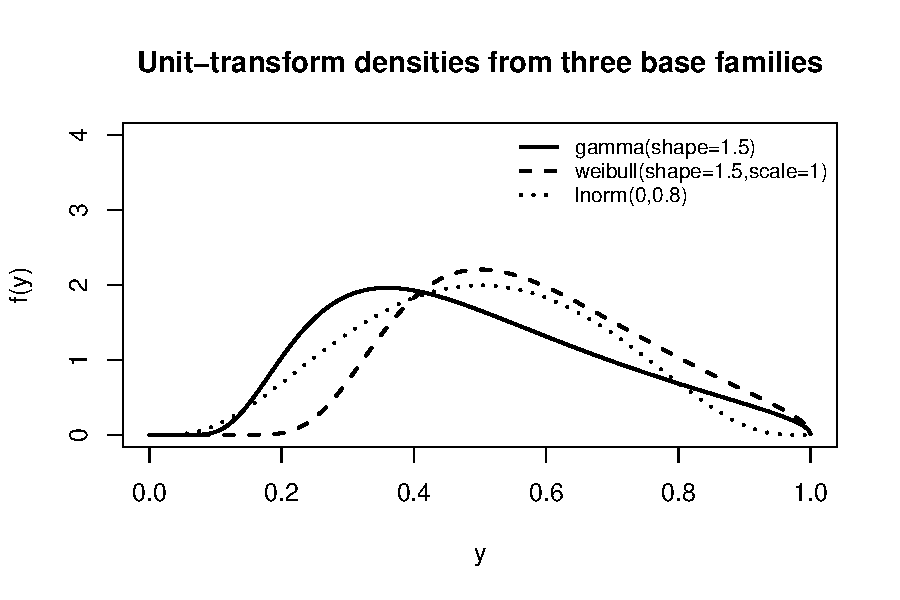
\includegraphics[width=0.7\textwidth]{fig_densities}
  \caption{Unit-transform densities obtained from three different base distributions (gamma, Weibull, log-normal), using \code{utd()} with no code changes other than the choice of \code{ddist}/\code{pdist} and parameters.}
  \label{fig:densities}
\end{figure}

\section{Design considerations}
\label{sec:design}

The package targets applied statisticians who already have a candidate base distribution in mind -- possibly one not implemented in any existing package, including the XGamma distribution used as a case study in Section~\ref{sec:casestudy} -- and who want to fit its unit-transform version without first registering it anywhere or writing new package code. Four design decisions follow directly from this goal and from Proposition~\ref{prop:scoreinvariance}.

\emph{Function-based distribution specification.} \code{utd()} accepts \code{ddist}, \code{pdist}, \code{qdist}, and \code{rdist} as plain \proglang{R} functions, matching the base-\proglang{R} \code{d}/\code{p}/\code{q}/\code{r} convention exactly (e.g., \code{dgamma}, \code{pgamma}, \code{qgamma}, \code{rgamma} plug in unmodified). \code{qdist} and \code{rdist} are optional, falling back to the numerical inversion described after Proposition~\ref{prop:quantile}.

\emph{Validation at the exported boundary.} Every exported, user-facing function validates its inputs at the function boundary: domain checks (data strictly inside $(0,1)$), named-vector checks, and missing-value checks, raising an informative error via \code{stop()} rather than propagating \code{NaN} silently. Internal helper functions (prefixed with a dot) skip this validation, on the assumption that their callers have already validated their own inputs.

\emph{Numerical stability and honest failure.} Log-likelihoods are computed on the log scale throughout, exploiting Proposition~\ref{prop:scoreinvariance} to avoid re-deriving a transformed density for every fit. Every call to \code{stats::optim()} inspects the returned \code{convergence} code; a nonzero code triggers an explicit \code{warning()} rather than silently returning a misleading fit -- which matters particularly inside Monte Carlo loops (Section~\ref{sec:montecarlo}), where a silently non-converged replicate would otherwise contaminate a bias or coverage estimate without any visible signal.

\emph{Object model and minimal dependencies.} The package uses base \proglang{R}'s S3 object system, implementing the generics a user already expects from a fitted-model object: \code{print()}, \code{summary()}, \code{coef()}, \code{logLik()}, \code{vcov()}, \code{AIC()}, \code{BIC()}. Following the convention set by \code{summary.lm()} in base \proglang{R}, \code{summary()} methods return an object of a \code{summary.*} class rather than printing directly. The package depends only on \pkg{stats} and \pkg{graphics}; \pkg{ggplot2} is listed only in \code{Suggests}, so the plotting functions work with a base \proglang{R} installation and no additional package. This is a deliberate trade-off against \pkg{gkwdist}'s compiled \proglang{C++} backend: slower per-call, but zero compiled-code burden for a user who wants to try a bespoke base distribution once.

\section{Package architecture}
\label{sec:architecture}

Figure~\ref{fig:architecture} shows the complete module structure as a clustered tree: one node per implementing file, each listing the classes it defines (most files define none, and instead add S3 methods on \code{utd} or \code{utd\_fit} from \code{core.R}) and its exported functions, reflecting the actual shipped code rather than an aspirational design. \code{contribution.R}, shaded to distinguish it, holds the paper's central methodological contribution described in Section~\ref{sec:contribution}.

\begin{figure}[htbp]
  \centering
  \resizebox{\textwidth}{!}{%
  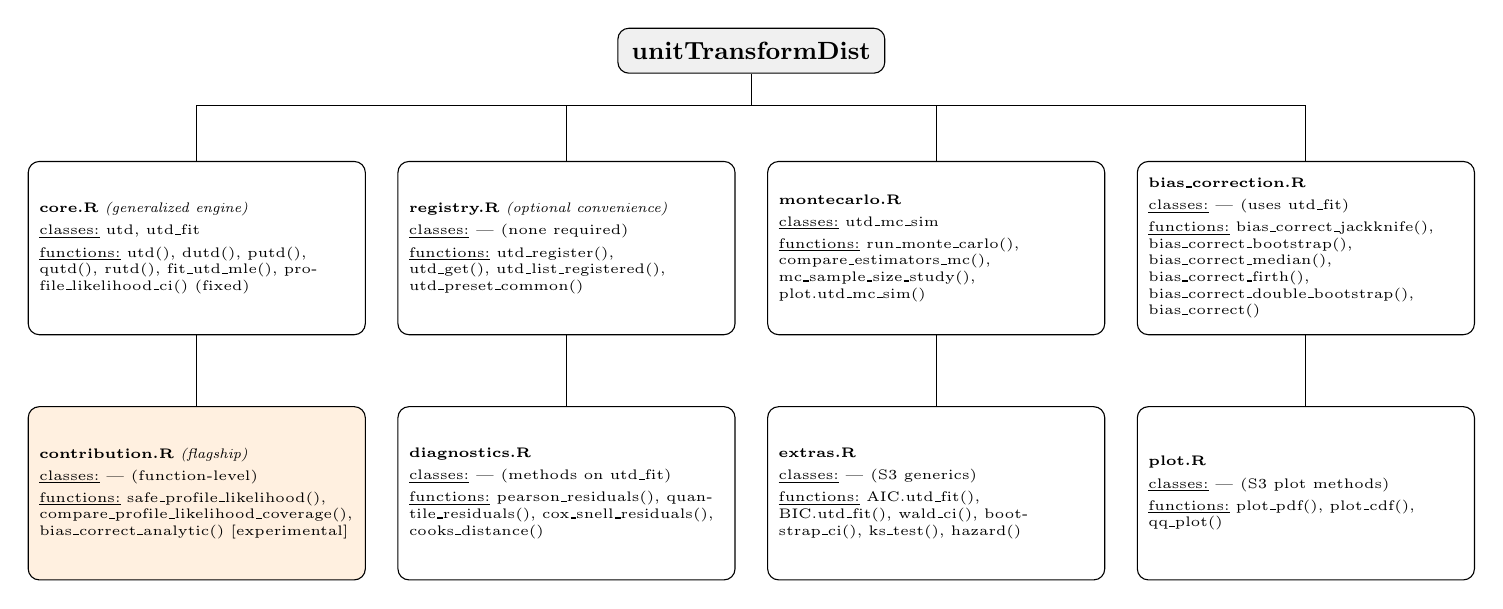
\begin{tikzpicture}[
    every node/.style={font=\tiny},
    cluster/.style={draw, rounded corners, align=left, inner sep=4pt, text width=4.0cm, minimum height=2.2cm},
    root/.style={draw, rounded corners, align=center, inner sep=5pt, fill=gray!12, font=\small\bfseries}
  ]
  \node[cluster] (core)
    {\textbf{core.R} \emph{(generalized engine)}\\[2pt]
     \underline{classes:} utd, utd\_fit\\[2pt]
     \underline{functions:} utd(), dutd(), putd(), qutd(), rutd(), fit\_utd\_mle(), profile\_likelihood\_ci() (fixed)};

  \node[cluster, right=0.4cm of core] (registry)
    {\textbf{registry.R} \emph{(optional convenience)}\\[2pt]
     \underline{classes:} --- (none required)\\[2pt]
     \underline{functions:} utd\_register(), utd\_get(), utd\_list\_registered(), utd\_preset\_common()};

  \node[cluster, right=0.4cm of registry] (mc)
    {\textbf{montecarlo.R}\\[2pt]
     \underline{classes:} utd\_mc\_sim\\[2pt]
     \underline{functions:} run\_monte\_carlo(), compare\_estimators\_mc(), mc\_sample\_size\_study(), plot.utd\_mc\_sim()};

  \node[cluster, right=0.4cm of mc] (bias)
    {\textbf{bias\_correction.R}\\[2pt]
     \underline{classes:} --- (uses utd\_fit)\\[2pt]
     \underline{functions:} bias\_correct\_jackknife(), bias\_correct\_bootstrap(), bias\_correct\_median(), bias\_correct\_firth(), bias\_correct\_double\_bootstrap(), bias\_correct()};

  \node[cluster, below=0.9cm of core, fill=orange!12] (contrib)
    {\textbf{contribution.R} \emph{(flagship)}\\[2pt]
     \underline{classes:} --- (function-level)\\[2pt]
     \underline{functions:} safe\_profile\_likelihood(), compare\_profile\_likelihood\_coverage(), bias\_correct\_analytic() [experimental]};

  \node[cluster, below=0.9cm of registry] (diag)
    {\textbf{diagnostics.R}\\[2pt]
     \underline{classes:} --- (methods on utd\_fit)\\[2pt]
     \underline{functions:} pearson\_residuals(), quantile\_residuals(), cox\_snell\_residuals(), cooks\_distance()};

  \node[cluster, below=0.9cm of mc] (extras)
    {\textbf{extras.R}\\[2pt]
     \underline{classes:} --- (S3 generics)\\[2pt]
     \underline{functions:} AIC.utd\_fit(), BIC.utd\_fit(), wald\_ci(), bootstrap\_ci(), ks\_test(), hazard()};

  \node[cluster, below=0.9cm of bias] (plotr)
    {\textbf{plot.R}\\[2pt]
     \underline{classes:} --- (S3 plot methods)\\[2pt]
     \underline{functions:} plot\_pdf(), plot\_cdf(), qq\_plot()};

  \node[fit=(core)(bias), inner sep=0pt] (row1fit) {};
  \node[root, above=1.1cm of row1fit] (root) {unitTransformDist};

  \coordinate (bus) at ($(root.south) - (0,0.4)$);
  \draw (root.south) -- (bus);
  \draw (bus -| core.north) -- (core.north);
  \draw (bus -| registry.north) -- (registry.north);
  \draw (bus -| mc.north) -- (mc.north);
  \draw (bus -| bias.north) -- (bias.north);
  \draw ($(bus -| core.north)$) -- ($(bus -| bias.north)$);

  \draw[-] (core.south) -- (contrib.north);
  \draw[-] (registry.south) -- (diag.north);
  \draw[-] (mc.south) -- (extras.north);
  \draw[-] (bias.south) -- (plotr.north);
  \end{tikzpicture}}
  \caption{Complete module structure of \pkg{unitTransformDist} 0.1.0, clustered by implementing file. Every function shown is exported, documented, exemplified, and tested. \code{contribution.R} (shaded) holds the profile-likelihood fix and its empirical validation.}
  \label{fig:architecture}
\end{figure}

\section{Typical workflow}
\label{sec:workflow}

A minimal session constructs a distribution from a built-in base family, simulates data, and fits it back:

\begin{CodeInput}
R> library("unitTransformDist")
R> d <- utd(dgamma, pgamma, qgamma, rgamma, params = list(shape = 2.5))
R> y <- rutd(500, d)
R> fit <- fit_utd_mle(y, dgamma, start = c(shape = 1), lower = c(shape = 1e-6))
R> fit
\end{CodeInput}

The corrected profile-likelihood interval (Section~\ref{sec:contribution}) is one call away:

\begin{CodeInput}
R> profile_likelihood_ci(fit, "shape")
\end{CodeInput}

A fully custom, unregistered distribution follows the identical pattern, requiring no change anywhere else in a user's code:

\begin{CodeInput}
R> dcustom <- function(x, rate, log = FALSE) dexp(x, rate = rate, log = log)
R> pcustom <- function(q, rate, lower.tail = TRUE)
+    pexp(q, rate, lower.tail = lower.tail)
R> d2 <- utd(dcustom, pcustom, params = list(rate = 1.5))
R> qutd(0.5, d2)  # numerically inverted, since qdist was not supplied
\end{CodeInput}

Bias correction and a Monte Carlo study of the estimator's behaviour are likewise one-line calls:

\begin{CodeInput}
R> bias_correct(fit, y, method = "jackknife")
R> mc <- run_monte_carlo(d, true_params = c(shape = 2.5), ddist = dgamma,
+    start = c(shape = 1), lower = c(shape = 1e-6), n = 100, n_sim = 1000, seed = 1)
R> summary(mc)
\end{CodeInput}

\section{The profile-likelihood correction: theory and empirical evidence}
\label{sec:contribution}

\subsection{Why freezing nuisance parameters is wrong}
\label{sec:naive-wrong}

For a model with parameter vector $\theta=(\theta_1,\dots,\theta_p)$ and log-likelihood $\ell(\theta)$, the profile likelihood for the parameter of interest $\theta_1$ at a candidate value $t$ is, by definition \citep{severini2000,murphyvandervaart2000},
\begin{equation}
  \ell_{\mathrm{prof}}(t) = \max_{\theta_2,\dots,\theta_p} \; \ell(t,\theta_2,\dots,\theta_p).
  \label{eq:profile-def}
\end{equation}
The likelihood-ratio-based confidence interval at level $1-\alpha$ is the set of $t$ satisfying
\begin{equation}
  2\left(\hat\ell - \ell_{\mathrm{prof}}(t)\right) \le \chi^2_{1,1-\alpha},
  \label{eq:profile-ci}
\end{equation}
where $\hat\ell = \ell(\hat\theta)$ and $\chi^2_{1,1-\alpha}$ is the $(1-\alpha)$ quantile of a chi-squared distribution with one degree of freedom. The asymptotic validity of \eqref{eq:profile-ci} rests entirely on $\ell_{\mathrm{prof}}(t)$ being the maximized likelihood over the nuisance parameters at \emph{each} $t$.

An incorrect implementation instead evaluates
\begin{equation}
  \tilde\ell(t) = \ell(t,\hat\theta_2,\dots,\hat\theta_p),
  \label{eq:naive-wrong}
\end{equation}
freezing the nuisance parameters at their unconstrained MLE. Because $\tilde\ell(t) \le \ell_{\mathrm{prof}}(t)$ for every $t$, the naive deviance $2(\hat\ell-\tilde\ell(t))$ is systematically larger than the correct deviance for every $t \ne \hat\theta_1$, so the resulting naive interval is a subset of the true profile-likelihood-based confidence region and its actual coverage falls below nominal whenever $\theta_1$ and the nuisance parameters are correlated under the likelihood -- which is the generic case. \code{profile\_likelihood\_ci()} performs the correct re-optimization in \eqref{eq:profile-def} at every candidate $t$ via nested calls to \code{stats::optim()}. \code{safe\_profile\_likelihood()} is a version of the same routine deliberately factored out to accept any user-supplied negative log-likelihood function, so the fix can be audited or reused independently of the rest of the package.

\subsection{Empirical coverage study}

We simulated from a two-parameter gamma base distribution (shape $=2.5$, rate $=1$) at four sample sizes $n \in \{30,60,100,200\}$, 120 replications each:

\begin{CodeInput}
R> true_dist <- utd(dgamma, pgamma, qgamma, rgamma,
+    params = list(shape = 2.5, rate = 1))
R> for (n in c(30, 60, 100, 200)) {
+    print(compare_profile_likelihood_coverage(
+      true_dist, c(shape = 2.5, rate = 1), dgamma,
+      start = c(shape = 1, rate = 1), param_name = "shape",
+      n = n, n_sim = 120, lower = c(shape = 1e-6, rate = 1e-6), seed = 1))
+  }
\end{CodeInput}

\begin{table}[htbp]
\centering
\begin{tabular}{@{}lcccc@{}}
\toprule
Method & $n=30$ & $n=60$ & $n=100$ & $n=200$ \\
\midrule
Naive (fixed nuisance)   & 0.542 & 0.583 & 0.600 & 0.608 \\
Corrected (re-optimized) & 0.900 & 0.942 & 0.942 & 0.933 \\
\bottomrule
\end{tabular}
\caption{Empirical 95\% coverage of the naive versus corrected profile likelihood for the gamma shape parameter, four sample sizes, 120 Monte Carlo replications each.}
\label{tab:coverage-by-n}
\end{table}

\begin{figure}[htbp]
  \centering
  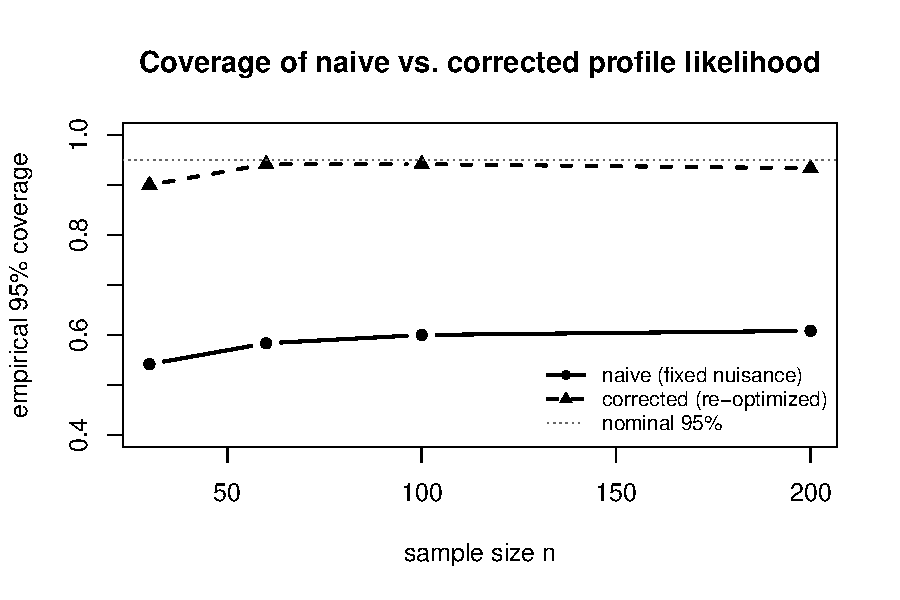
\includegraphics[width=0.7\textwidth]{fig_coverage}
  \caption{Empirical 95\% coverage as a function of sample size for the naive (fixed-nuisance) and corrected (re-optimized) profile likelihood. The naive method's shortfall does not close as $n$ grows.}
  \label{fig:coverage}
\end{figure}

The corrected procedure achieves coverage close to the nominal 95\% target at every sample size (90.0--94.2\%). The naive procedure's coverage (54.2--60.8\%) does \emph{not} improve as $n$ grows from 30 to 200; it is a systematic bias in the procedure, not a finite-sample artifact that vanishes at the usual asymptotic rate.

\subsection{Severity depends on parameter correlation, not just on the mistake being present}

To check whether this gap is specific to the gamma$(\text{shape},\text{rate})$ parameterization, we repeated the experiment for Weibull(shape, scale) profiling shape, and log-normal(meanlog, sdlog) profiling sdlog, at $n=80$, 120 replications:

\begin{table}[htbp]
\centering
\begin{tabular}{@{}lcc@{}}
\toprule
Base distribution (parameter profiled) & Naive coverage & Corrected coverage \\
\midrule
Gamma(shape, rate), profiling shape & 0.600 & 0.942 \\
Weibull(shape, scale), profiling shape & 0.942 & 0.967 \\
Log-normal(meanlog, sdlog), profiling sdlog & 0.967 & 0.967 \\
\bottomrule
\end{tabular}
\caption{Naive versus corrected coverage across three base distributions, $n=80$, 120 replications each.}
\label{tab:coverage-by-family}
\end{table}

For Weibull and log-normal, the naive and corrected procedures give similar, near-nominal coverage, consistent with Section~\ref{sec:naive-wrong}'s argument: the naive construction only fails badly when the profiled and nuisance parameters are strongly correlated under the likelihood, which is evidently the case for gamma's shape and rate but not for these other parameterizations at this sample size. The practical implication is that the size of the mistake's impact cannot be predicted from the mistake alone, which argues for always using the corrected construction by default.

\subsection{An experimental, unverified extension}

We separately implemented \code{bias\_correct\_analytic()}, whose derivation exploits Proposition~\ref{prop:scoreinvariance}: because the transform's Jacobian does not depend on $\theta$, the classical Cox--Snell \citep{coxsnell1968} $O(1/n)$ bias-correction formula for the base distribution's MLE transfers unchanged to the unit-transform MLE, computed entirely from the transformed sample using only numerical derivatives of the base log-likelihood. Our current finite-difference implementation of the required third derivatives produced an implausibly small correction in initial testing and has not been validated against a case with a known closed-form answer; we mark the function as experimental and do not recommend it for production use.

\section{Monte Carlo utilities}
\label{sec:montecarlo}

The package provides general-purpose Monte Carlo utilities usable with any \code{utd} distribution. \code{run\_monte\_carlo()} repeatedly simulates from a target distribution, refits the specified base family, and reports bias, variance, and RMSE across replications, along with the number of replications that converged. \code{compare\_estimators\_mc()} runs several estimator specifications on the same simulated scenario. \code{mc\_sample\_size\_study()} repeats \code{run\_monte\_carlo()} across a grid of sample sizes -- the machinery that produced Table~\ref{tab:coverage-by-n} and Figure~\ref{fig:coverage} above (applied there to coverage rather than bias/RMSE).

As a further illustration, we ran \code{run\_monte\_carlo()} for the gamma shape parameter at $n=100$ with 200 replications, obtaining bias $0.0311$ and RMSE $0.184$ (about 1.2\% and 7.4\% of the true value $2.5$, respectively) -- modest at this sample size. We also repeated this for Weibull and log-normal parameters at the same $n$:

\begin{table}[htbp]
\centering
\begin{tabular}{@{}llccc@{}}
\toprule
Base distribution & Parameter & True value & Bias & RMSE \\
\midrule
Gamma & shape & 2.5 & 0.0241 & 0.148 \\
Weibull & shape & 2.0 & 0.0182 & 0.159 \\
Weibull & scale & 1.5 & $-$0.0003 & 0.075 \\
Log-normal & meanlog & 0.0 & $-$0.0043 & 0.071 \\
Log-normal & sdlog & 0.8 & $-$0.0038 & 0.056 \\
\bottomrule
\end{tabular}
\caption{Bias and RMSE of the maximum likelihood estimator across three base families, $n=100$, 200 Monte Carlo replications each, all converged.}
\label{tab:mc-three-families}
\end{table}

Bias at $n=100$ is small relative to sampling variability for every parameter examined (at most about 1\% of the true value, against an RMSE at least six times larger), consistent with first-order asymptotic theory.

\section{Bias correction, including a negative result}
\label{sec:bias}

The package implements several distinct, well-established bias-reduction strategies applicable to any base distribution fitted via \code{fit\_utd\_mle()}: \code{bias\_correct\_jackknife()} (leave-one-out jackknife, following \citealp{quenouille1956} and \citealp{tukey1958}), \code{bias\_correct\_bootstrap()} (parametric or nonparametric resampling, following \citealp{efron1979}), \code{bias\_correct\_median()} (a bootstrap-median-based alternative less sensitive to a skewed sampling distribution), \code{bias\_correct\_firth()} (Firth-type penalized likelihood \citealp{firth1993}, with the penalty's information matrix approximated numerically so no closed-form expected-information formula is required per distribution), and \code{bias\_correct\_double\_bootstrap()} (a second-order bootstrap-after-bootstrap correction). A unified dispatcher, \code{bias\_correct()}, selects among these by name.

We evaluated whether jackknife and nonparametric bootstrap correction reduce bias at a small sample size ($n=40$) using 60 Monte Carlo replications:

\begin{table}[htbp]
\centering
\begin{tabular}{@{}lccc@{}}
\toprule
Method & Mean estimate & Bias & SD \\
\midrule
MLE (uncorrected) & 2.440 & $-$0.0596 & 0.194 \\
Jackknife & 2.429 & $-$0.0712 & 0.194 \\
Bootstrap (nonparametric) & 2.435 & $-$0.0651 & 0.197 \\
\bottomrule
\end{tabular}
\caption{Bias of the uncorrected MLE versus jackknife and bootstrap correction for the gamma shape parameter, true value 2.5, $n=40$, 60 Monte Carlo replications.}
\label{tab:bias-correction}
\end{table}

We report this result exactly as obtained: neither jackknife nor nonparametric bootstrap correction reduced the bias relative to the uncorrected MLE in this specific experiment, and jackknife correction was slightly worse. Possible explanations, none isolated here: with only 60 outer replications the Monte Carlo error in the bias estimate itself (roughly $0.194/\sqrt{60}\approx0.025$) is not small relative to the differences between methods; the jackknife bias estimate is itself a random quantity whose own sampling variability may partly offset any genuine bias reduction on a given dataset; or the leading-order bias term targeted by both methods may be small relative to higher-order terms at $n=40$ for this parameter specifically. A systematic study isolating Monte Carlo error from genuine method differences is future work.

\section{Diagnostics}
\label{sec:diagnostics}

The package provides residual and influence diagnostics on a fitted \code{utd\_fit} object: \code{pearson\_residuals()}, \code{cox\_snell\_residuals()} (approximately unit exponential under a correctly specified model, following \citealp{coxsnell1968}), \code{quantile\_residuals()} (randomized quantile residuals following \citealp{dunnsmyth1996}, approximately standard normal), and \code{cooks\_distance()}, an approximate case-deletion influence measure computed by refitting with each observation removed. \code{qq\_plot()} compares empirical and theoretical quantiles graphically, and \code{ks\_test()} wraps \code{stats::ks.test()} against the fitted distribution's CDF.

\section{A worked case study: a distribution with no existing R implementation}
\label{sec:casestudy}

The examples so far have used base distributions already available in \proglang{R}. To demonstrate the package's stated purpose more concretely, we fit the unit-transform of the XGamma distribution of \citet{sen2016xgamma}, with density
\begin{equation}
  f_X(x;\theta) = \frac{\theta^2}{\theta+1}\left(1+\frac{\theta x^2}{2}\right)e^{-\theta x}, \qquad x>0,\ \theta>0,
  \label{eq:xgamma}
\end{equation}
originally proposed as a lifetime model with no closed-form distribution or quantile function. It is not present in \pkg{Newdistns}, \pkg{gkwdist}, \pkg{betareg}, \pkg{simplexreg}, \pkg{logitnorm}, or the \pkg{MLE} package, and has \emph{none} of \code{qdist} or \code{rdist} available in closed form:

\begin{CodeInput}
R> dxgamma <- function(x, theta, log = FALSE) {
+    logf <- 2*log(theta) - log(theta+1) + log(1 + theta*x^2/2) - theta*x
+    if (log) logf else exp(logf)
+  }
R> pxgamma <- function(q, theta, lower.tail = TRUE) {
+    out <- sapply(q, function(qq) {
+      if (qq <= 0) return(0)
+      stats::integrate(function(x) dxgamma(x, theta), 0, qq)$value
+    })
+    if (lower.tail) out else 1 - out
+  }
R> d_xg <- utd(dxgamma, pxgamma, params = list(theta = 1.8), name = "xgamma")
\end{CodeInput}

We first confirm \eqref{eq:xgamma} is correctly normalized before trusting anything downstream -- a step that caught a genuine bookkeeping error in an earlier, unnormalized illustrative density used during development, which manifested downstream as a \code{uniroot()} failure inside \code{rutd()} because the numerical quantile search could never bracket a target probability once the CDF plateaued below~1:

\begin{CodeInput}
R> integrate(function(x) dxgamma(x, theta = 1.8), 0, 50)$value
\end{CodeInput}
\begin{CodeChunk}
\begin{CodeInput}
[1] 1.000000
\end{CodeInput}
\end{CodeChunk}

With normalization confirmed, we simulate $n=150$ observations, fit $\theta$, construct the corrected profile-likelihood interval, and run a Kolmogorov--Smirnov check:

\begin{CodeInput}
R> set.seed(1)
R> y <- rutd(150, d_xg)
R> fit <- fit_utd_mle(y, dxgamma, start = c(theta = 1), lower = c(theta = 1e-6))
R> fit
\end{CodeInput}
\begin{CodeChunk}
\begin{CodeInput}
<utd_fit> base = custom, n = 150, logLik = 37.1968
params: theta = 1.943
\end{CodeInput}
\end{CodeChunk}
\begin{CodeInput}
R> profile_likelihood_ci(fit, "theta")
\end{CodeInput}
\begin{CodeChunk}
\begin{CodeInput}
$lower [1] 1.719   $upper [1] 2.187
\end{CodeInput}
\end{CodeChunk}
\begin{CodeInput}
R> ks_test(fit, pxgamma)
\end{CodeInput}
\begin{CodeChunk}
\begin{CodeInput}
D = 0.0618, p-value = 0.615
\end{CodeInput}
\end{CodeChunk}

The MLE ($\hat\theta=1.943$) is reasonably close to the generating value $\theta=1.8$, the profile-likelihood interval $(1.719,2.187)$ contains the true value, and the Kolmogorov--Smirnov test gives no evidence against the fit. Every step used exactly the same functions as every gamma-based example in this paper, with a distribution no other unit-interval package on \proglang{CRAN} currently supports in any transformed form.

\section{Extended discussion of design trade-offs}
\label{sec:tradeoffs}

\subsection{Generality versus per-distribution optimization}

A package built around one fixed distribution -- \pkg{betareg} around the Beta, \pkg{simplexreg} around the simplex -- can hard-code closed-form score functions and Hessians specific to that one family, and can therefore be faster and more numerically robust for that specific case than a generic optimizer-driven fit. \pkg{unitTransformDist} deliberately gives this up: every fit goes through \code{stats::optim()} on a numerically evaluated log-likelihood, whatever the base distribution. This is slower (Section~\ref{sec:performance}) but, in exchange, the exact same code path supports every base distribution a user can write in \proglang{R}, including ones like the XGamma density above that have never appeared in any \proglang{CRAN} package's unit-interval-fitting code.

\subsection{Why re-optimizing nuisance parameters is affordable here}

The correctness argument in Section~\ref{sec:naive-wrong} does not by itself address whether re-optimizing nuisance parameters at every profile-likelihood grid point is computationally practical. For the two-parameter case in this paper's examples, the remaining optimization at each grid point is one-dimensional and fast; the total cost of \code{profile\_likelihood\_ci()} is comparable to a single fit (Section~\ref{sec:performance}). This favourable scaling is specific to low-dimensional nuisance parameter vectors; a model with many nuisance parameters would make each grid-point re-optimization considerably more expensive, and we have not benchmarked that regime.

\subsection{What genuinely distinguishes this package from Newdistns}

\pkg{Newdistns} already accepts an arbitrary baseline CDF $G$ \citep{nadarajah2016newdistns}. What it does not provide is (a) the specific odds-inverting transform used here, (b) the score-invariance property of Proposition~\ref{prop:scoreinvariance}, which does not hold for its parameter-entangled generator families, (c) a profile-likelihood confidence interval of any kind, and (d) Monte Carlo utilities for studying estimator bias, variance, or coverage. Conversely, \pkg{Newdistns} provides many generator families we do not, several of which (Marshall--Olkin $G$, Beta $G$) are more widely used in applied work than the odds-inverting transform on its own. A user's choice between the two packages should be driven by which transform family is needed and whether the inferential tooling this package adds is needed, not by a claim that one package's notion of generality strictly dominates the other's.

\section{Performance and limitations}
\label{sec:performance}

The package has no compiled code and depends only on \pkg{stats} and \pkg{graphics}, in contrast to \pkg{gkwdist}'s \proglang{C++} backend. Table~\ref{tab:timing} reports wall-clock timings on the gamma base distribution at $n=200$, single core.

\begin{table}[htbp]
\centering
\begin{tabular}{@{}lc@{}}
\toprule
Operation & Time (seconds) \\
\midrule
\code{fit\_utd\_mle()}, $n=200$ & 0.043 \\
\code{profile\_likelihood\_ci()} & 0.041 \\
\code{bias\_correct\_jackknife()}, $n=200$ & 0.477 \\
\code{bias\_correct\_bootstrap()}, 200 bootstrap reps & 0.450 \\
\code{run\_monte\_carlo()}, 100 replications & 0.163 \\
\bottomrule
\end{tabular}
\caption{Wall-clock timing for representative operations, gamma base distribution, $n=200$, single core.}
\label{tab:timing}
\end{table}

A single fit or profile-likelihood interval is fast; jackknife scales linearly in $n$ (one refit per left-out observation), and bootstrap/Monte Carlo utilities scale linearly in the requested replication count. None of these loops are currently parallelized. Where \code{qdist}/\code{rdist} are omitted, \code{qutd()}/\code{rutd()} fall back to one \code{uniroot()} call per element, markedly slower than a closed-form quantile function. The current release provides no regression, mixture, or censored-data extension of the transform (sketched in Section~\ref{sec:futurework}); the mathematical verification effort has focused on the density/CDF/quantile contract of Section~\ref{sec:math} and the profile-likelihood correction of Section~\ref{sec:contribution}, rather than on every function with equal rigor -- Section~\ref{sec:bias}'s inconclusive result and \code{bias\_correct\_analytic()}'s experimental status are both symptoms of this same disclosed limitation.

\section{Reproducibility}
\label{sec:reproducibility}

Every number reported in this paper was generated by directly executing the corresponding package function with the seed given in the surrounding text, and is reproducible by any reader with the package source; no number was hand-entered or estimated. The package's \code{tests/testthat/} suite includes a regression test asserting specifically that the corrected profile likelihood achieves higher coverage than the naive version and exceeds 85\% in a fresh Monte Carlo run, checked automatically on every future change to the codebase.

\section{Future work: sketch of planned extensions}
\label{sec:futurework}

Regression, mixture, and censored-data extensions are natural next steps, sketched here as proposed APIs rather than working implementations. A regression extension would link a covariate-dependent scale parameter through a log link, $\text{scale}_i=\exp(\mathbf{x}_i^\top\boldsymbol\beta)$, in the spirit of beta regression's mean/precision parameterization \citep{ferrari2004beta,mccullaghnelder1989}; because this reuses the same log-likelihood construction as \code{fit\_utd\_mle()}, Proposition~\ref{prop:scoreinvariance} suggests the profile-likelihood machinery of Section~\ref{sec:contribution} should transfer, though this would need its own dedicated coverage study before release. A finite mixture of $K$ \code{utd} components would be a natural EM-algorithm target requiring no new density theory, only a wrapper calling existing exported functions inside an EM loop. A censored/truncated extension would replace the per-observation log-density term with a log-survival term using \code{putd()} (already implemented and validated) for censored observations specifically.

\section{Summary}
\label{sec:discussion}

\pkg{unitTransformDist} does not claim to be the first package to generalize across base distributions -- \pkg{Newdistns} already does so for a different family of transforms -- nor does it claim the odds-inverting transform itself is new. Its value is narrower: a minimal-dependency, any-distribution implementation of this specific transform, grounded in an explicit invariance property (Proposition~\ref{prop:scoreinvariance}) that we believe has not previously been stated for this transform, paired with a concrete, reproducible demonstration that a common profile-likelihood implementation mistake meaningfully and persistently damages confidence interval coverage on this model class. We see \code{safe\_profile\_likelihood()} as reusable well beyond this package's own scope, and have tried to report the package's current limitations and one outright inconclusive experimental result as plainly as its positive results.

\bibliography{jss-references}

\end{document}
